\documentclass[twoside,a4paper]{book}
\usepackage{graphicx}
\usepackage{hyperref}
\usepackage{amsmath}
\usepackage{amssymb}
\usepackage{textcomp}
\usepackage[utf8]{inputenc}
\usepackage[polish]{babel}
\usepackage[T1]{fontenc}
\usepackage{standalone}
\usepackage{array}
% pakiet stosowany do url'i w bibliografii, zamienia odnośniki na ładnie sformatowane
\usepackage{url}
% pakiety służące do numerowania i tworzenia algorytmów
\usepackage{algorithmic}
\usepackage{algorithm}
\makeatletter
\renewcommand{\ALG@name}{Algorytm}
\makeatother
% redefinicja etykiety nagłówkowej listy algorytmów, domyślna jest po angielsku
\renewcommand{\listalgorithmname}{Spis algorytmów}

\usepackage[section]{placeins}
\usepackage{pdfpages}

% pakiet do wyliczania skali, przydatny przy dużych obrazkach
\usepackage{pgf}
% pakiet służący do automatycznego sortowania odnośników do bibliografii
\usepackage[sort]{natbib}
% tworzenie listingów
\usepackage{listings}
% tworzenie figur wewnątrz figur
\usepackage{subfig}
% do automatycznego skracania nazw rozdziałów i podrozdziałów używanych w nagłówkach strony by mieściły się w jednej linii
\usepackage[fit]{truncate}
% fancyhdr - ładne nagłówki, definicja wyglądu nagłówka, numery stron będą umieszczane w nagłówku po odpowiedniej stronie
\usepackage{fancyhdr}
\pagestyle{fancy}
\renewcommand{\chaptermark}[1]{\markboth{#1}{}}
\renewcommand{\sectionmark}[1]{\markright{\thesection\ #1}}



\fancyhf{}
\fancyhead[LE,RO]{\bfseries\thepage}
% tutaj ograniczamy szerokość pola w nagłówku zawierającego nazwę rozdziału/podrozdziału do 95% szerokości strony
% redefinicja sposobu prezentacji nazw domyślnie wypisywanych wielkimi literami (np. domyślnie w nagłówku Spis treści będzie miał postać SPIS TREŚCI)
% Uwaga! to może popsuć wielkie litery w ogóle! Jak coś nie działa należy usunąć \nouppercase{} z poniższych definicji
\fancyhead[LO]{\nouppercase{\bfseries{\truncate{.95\headwidth}{\rightmark}}}}
\fancyhead[RE]{\nouppercase{\bfseries{\truncate{.95\headwidth}{\leftmark}}}}
\renewcommand{\headrulewidth}{0.5pt}
\renewcommand{\footrulewidth}{0pt}

% definicja typu prostego wymagana przez pierwsze strony rozdziałów itp.
% powyższe reguły niestety tych stron nie dotyczą, gdyż Latex automatycznie przełącza je pomiędzy fancy a plain
% w tym wypadku eliminujemy nagłówki i stopki na stronach początkowych
\fancypagestyle{plain}{%
 \fancyhead{}
 \fancyfoot{}
 \renewcommand{\headrulewidth}{0pt}
 \renewcommand{\footrulewidth}{0pt}
}

\parskip 0.05in


% makro umożliwiające otaczanie symboli okręgami
\usepackage{tikz}
% brak justowania tekstu (bazą okręgu będzie linia tekstu)
\newcommand*\mycirc[1]{%
  \begin{tikzpicture}
    \node[draw,circle,inner sep=1pt] {#1};
  \end{tikzpicture}}

% pionowe justowanie tekstu, środek okręgu pokrywa się ze środkiem tekstu
\newcommand*\mycircalign[1]{%
  \begin{tikzpicture}[baseline=(C.base)]
    \node[draw,circle,inner sep=1pt](C) {#1};
  \end{tikzpicture}}

% zmiana nazwy twierdzeń i lematów
\newtheorem{theorem}{Twierdzenie}[section]
\newtheorem{lemma}[theorem]{Lemat}

% tworzenie definicji dowodu
\newenvironment{proof}[1][Dowód]{\begin{trivlist}
\item[\hskip \labelsep {\bfseries #1}]}{\end{trivlist}}
% \newenvironment{definition}[1][Definicja]{\begin{trivlist}
% \item[\hskip \labelsep {\bfseries #1}]}{\end{trivlist}}
% \newenvironment{example}[1][Przykład]{\begin{trivlist}
% \item[\hskip \labelsep {\bfseries #1}]}{\end{trivlist}}
% \newenvironment{remark}[1][Uwaga]{\begin{trivlist}
% \item[\hskip \labelsep {\bfseries #1}]}{\end{trivlist}}

% definicja czarnego prostokąta zwyczajowo dodawanego na koniec dowodu
\newcommand{\qed}{\nobreak \ifvmode \relax \else
      \ifdim\lastskip<1.5em \hskip-\lastskip
      \hskip1.5em plus0em minus0.5em \fi \nobreak
      \vrule height0.75em width0.5em depth0.25em\fi}

% poniższymi instrukcjami można sterować co ma być numerowane a co nie i co ma być wyświetlane w spisie treści
% \setcounter{secnumdepth}{3}
% \setcounter{tocdepth}{5}

% definicja czcionki mniejszej niż tiny (domyślnie takiej małej nie ma)
\usepackage{lmodern}
\makeatletter
  \newcommand\tinyv{\@setfontsize\tinyv{4pt}{6}}
\makeatother

% definicja jeszcze mniejszej czcionki
\usepackage{lmodern}
\makeatletter
  \newcommand\tinyvv{\@setfontsize\tinyvv{3.5pt}{6}}
\makeatother

% pakiet do obsługi wielostronicowych tabel
\usepackage{longtable}
\setlength{\LTcapwidth}{\textwidth}

\usepackage[section] {placeins}


\usepackage{multirow}

\usepackage{slantsc}
\usepackage[labelsep=endash]{caption}
\addto\captionspolish{\renewcommand{\figurename}{Rys.}}
\addto\captionspolish{\renewcommand{\tablename}{Tab.}}
\addto\captionspolish{\renewcommand*{\appendixpagename}{Dodatki}}
\addto\captionspolish{\renewcommand*{\appendixtocname}{Dodatki}}
\addto\captionspolish{\renewcommand*{\appendixname}{Dodatek}}
%\addto\captionspolish{\renewcommand{\algorthmcfname}{Algorytm: }}
\setcounter{secnumdepth}{5}

\usepackage[toc,page]{appendix}


\begin{document}
\chapter{Zaimplementowane algorytmy}
W poniższych podrozdziałach zaprezentowano zasadę działania zaimplemenetowanych w oprogramowaniu algorytmów. 
\section{Działanie przycisków}
W aplikacji każdy przycisk jest obiektem klasy ButtonOperator, która dziedziczy po klasie QPushButton. Dzięki czemu fizyczne obiekty przycisków mogą korzystać zarówno z metod klasy nadrzędnej np. isCheckable(), jak i klasy dziedziczącej. Właśnie dzięki nadpisaniu metod domyślnych klasy QPushButton  -  hoverEnter() i hoverLeave() stworzono możliwość detekcji, nad którym przyciskiem aktualnie znajduje się punkt fiksacji wzroku. Podczas wywołania obu metod zmieniana jest wartość logiczna zmiennej isHovered aktualnie obserwowanego przycisku.  Prócz informacji o tym, czy dany przycisk jest aktualnie używany przechowuje się również dane o tym, czy przycisk zalicza się do tkzw. ''specjalnych'', czy też nie, jak i listę dostępnych dla niego tekstów do wyświetlania – wyglądów przycisku dla 6 stanów klawiatury (małe litery, duże litery, znaki specjalne karta pierwsza, znaki specjalne karta druga, polskie litery, menu kontekstowe). Wszystkie te dane wprowadza się podczas  uruchamiania klawiatury i wtedy także zapisuje się przyciski kolejno do specjalnej listy. Kolejność jest znacząca w przypadku przycisków ''specjalnych'', gdyż ich obsługa zależna jest od wartości ich ID zapisanego w pliku ze stałymi. 
Określenie przycisku działającego odbywa się poprzez sprawdzenie ID przycisku, którego zmienna isHovered jest prawdziwa w klasie TimeManager. Do zarządzania stanem klawiatury, ostatnio wybranym przyciskiem specjalnym oraz ostatnio obserwowanym przyciskiem powstała klasa HoverManager. Zbiera ona na bieżąco informacje o  ID przycisku ostatnio najechanego, o tym przez jaki czas dany przycisk jest już pod punktem fiksacji, o aktualnym stanie klawiatury, o ostatnio wybranym specjalnym przycisku (np. CapsLock) oraz przez jaki czas działanie tego przycisku się utrzymuje. Większość z tych danych odświeżana jest co 200ms (stała zdefiniowana w pliku ze stałymi) podczas każdego wykonywania się metody TimerStep(). Jej działanie przedstawiono za pomocą pseudokodu ~\ref{sec:alg1}.
\begin{algorithm}
\caption{Działanie funkcji TimerStep()}
\label{sec:alg1}
\begin{algorithmic}
\STATE pobierz ID aktualnie fiksowanego przycisku
\IF{pobrane ID różne jest od -1}
\IF{zwykłe przyciski są w trybie wstrzymania}
\IF{jeśli aktualnie fiksowany przycisk jest specjalny}
\STATE hoverState (obiekt klasy HoverManager) ustaw aktualnie aktywny przycisk na pobrane ID
\STATE Wykonaj krok timera (funkcja executeTimerStep())
\STATE Pokaż czas przez jaki przycisk jest fiksowany na pasku postępu dla informacji użytkownika.
\ENDIF
\ELSE
\STATE Wykonaj powyższe funkcje dla wszystkich przycisków - niezależnie od tego, czy są specjalne, czy nie.
\ENDIF
\ENDIF
\STATE Wywołaj funkcję verifyTimerTickCount().
\end{algorithmic}
\end{algorithm}
\\Zadaniem wyżej wspomnianej funkcji executeTimerStep() jest sprawdzenie, czy dany przycisk był fiksowany przez odpowiednią ilość czas (zmienna, której wartość zależy od ilości pomyłek popełnionych przez użytkownika i dynamicznie zmieniana podczas korzystania z klawiatury – analizowane to jest w funkcji verifyTimerTickCount()). Jeżeli warunek ten został spełniony to dalszy przebieg działań zależy od tego, czy przycisk był specjalny, czy też nie oraz czy klawiatura nie znajduje się w trybie wstrzymania. 
\subsection{Działanie przycisków specjalnych}
W tabeli ~\ref{table:specialButtons} wymieniono wszystkie specjalne przyciski z widoku klawiatury oraz opisano po krótce algorytm ich działania. W tabeli ~\ref{table:specialButtonsMenu} przedstawiono przyciski widoku menu oraz ich zachowania.

\begin{table}
    \begin{tabular}{|p{4cm}|p{8.5cm}|}
        \hline
    \textbf{Nazwa przycisku} & \textbf{Działanie}\\ \hline
     Backspace & Wywołuję metodą backspace() klasy Dictionary WIĘCEJ W OBSŁUGA TESKTU\\ \hline
    CapsLock & W przypadku pierwszego wciśnięcia zmienia stan klawiatury z 0 na 1 i utrzymuje ją dopóki nie zostanie wybrany po raz wtóry lub wykonana zostanie czynność innego przycisku zmieniającego stan klawaiatury. \\ \hline
 Czyść & Korzysta z metody resetAll() klasy Dictionary i powoduje czyszczenie edytora tekstowego oraz z nim związanych zmiennych jak currentPosition, currentWord, currentWordSart, wholeTxt (więcej na ten temat w rodziale ~\ref{sec:text}).\\ \hline
Menu & Otwiera okno klasy Personalize.\\ \hline
Przesuń się o jedno słow w prawo lub w lewo & Wywołuje funkcje jumpWord() klasy Dictionary, która powoduje przesunięcie się kursora na koniec poprzedniego słowa, lub na początek kolejnego. Każdorazowo zmieniana jest wartość zmiennej currentWord i wholeText.~\ref{sec:text}\\ \hline
 Przesuń się w kierunku początku tekstu (home) lub na jego koniec (end) & Wybranie przycisku powoduje przesunięcie się kursora w jednym z dwóch kierunków oraz zmiane wartości zmiennej wholeText i currentWord (~\ref{sec:text}). \\ \hline
 Przyciski podpowiedzi & Wyświetlane na nich są podpowiedzi, których tworzenie jest opisane w rodziale ~\ref{sec:trietree}. Ich użycie powoduje zastąpienie aktualnie wpisywanej frazy auto uzupłenionym słowem pobranym ze słownika. \\ \hline
  Shift & W przypadku wciśnięcia zmieniony zostaje stan klawaiatury z 0 na 1, a po użyciu przycisku ze znakiem stan klawiatury wraca do stanu 0. \\ \hline
   Stop i start & Wprowadza klawaiturę w stan wstrzymania lub w stan pracy. W zależności od wartości zmiennej isStop możliwe,lub nie, jest korzystanie z przycisków ze znakami.\\ \hline
   Strzałka w lewo i prawo &  Korzystając z metody moveCursor klasy Dictionary przemieszcza kursor o jeden znak w danym kierunku. Może zmienić wartość currentWord (~\ref{sec:text}) korzystając z metod getCurrentWord() oraz getCurrentWordStart()(~\ref{sec:alg2}) opisanych w późniejszych rozdziałach.\\ \hline
     Wyjdź & Powoduje opuszczenie aplikacji.\\ \hline 
      Wyszukaj na podanej platformie & Przyciśniecie przycisku powoduje sprawdzenie połączenia internetowego, a następnie wysłanie wpisanej treści pola tekstowego do funkcji search() klasy GoogleSearcher. TUTAJ ODSYŁNIK DO KLASY\\ \hline
        Wyślij & Wysyła dotychczas wpisany tekst na broadcast na port 45454 za pomocą metody writeDatagram() klasy QUdpSocket.\\ \hline
    Zmiana trybu wyszukiwania & Strzałki powodują na zmianę trybu wyszukiwania. Do wyboru ''Google'', ''YouTube'', ''Filmweb''. Zmieniają wartość zmiennej sendingState niezbędnej do popranego działania funkcji  search() klasy GoogleSearcher.TUTAJ ODSYŁNIK DO KLASY\\ \hline 
    Znaki specjalne & Zmiania stan klawiatury na odpowiednio 2 i 3 przy kolejnych kliknięciach. \\ \hline
       \end{tabular}
    \caption{Lista specjalnych przycisków w raz z ich działaniem.} 
    \label{table:specialButtons}
\end{table}

\begin{table}
    \begin{tabular}{|p{4cm}|p{8.5cm}|}
        \hline
    \textbf{Nazwa przycisku} &. \textbf{Działanie}\\ \hline
       Strzałki zmieniające aktualną wartość progową czasu fiksacji & Strzałki powodują zmniejszenie lub zwiększenie wartości zmiennej tickCounter przechowującej ilość 200ms interwałów, po upływie których (w przypadku braku zmiany fiksowanego punktu) przycisk można uznać za wciśnięty. Początkowo czas ten wynosi 3s, jednak w wyniku dynamicznej korekty następującej, gdy użytkownik wykona mniej, lub więcej niż 5 błędów w ciągu minuty (średnio 25\%błednie wpisanych znaków), następuje zmniejszenie lub zwiększenie liczny tych interwałów. \\ \hline  
       Strzałki zmieniajace wielkość czcionki w edytorze tekstu & Strzałki powodują zamianę właściwości edytora tekstu. \\ \hline
       Strzałki zmieniające wygląd aplikacji & Użytkownik może wybrać między jednym z 5 wersji kolorystycznych poprzez dynamiczą zmianę wyglądu na podstawie danych z listy i aktualnego indeksu.  \\ \hline    
       Wyjście & Powoduje zamknięcie okna menu. \\ \hline
    \end{tabular}
    \caption{Lista specjalnych przycisków z menu w raz z ich działaniem.} 
    \label{table:specialButtonsMenu}
\end{table}


Jako wciśnięcie rozumie się tu czas fiksacji nad przyciskiem przekracający progową wartość. Stany klawiatury to odpowiednio 0-małe litery, 1-wielkie litery, 2-znaki specjalne strona pierwsza, 3-zanki specjalne strona druga, 4-polskie znaki, 5-menu kontekstowe dla polskich znaków.
\subsection{Działanie przycisków nomalnych}
Za wpisywanie znaków z klawiatury do edytora odpowiedzialna jest funkcja update() klasy Dictionary. Jest ona głównym zarządcą jeśli chodzi o wprowadzanie znaków w odpowiedniej pozycji. W pierwszym rzędzie sprawdzane jest, czy stan klawiatury różny jest od piątego (menu kontekstowe). Gdy spełniony jest dany warunek to porównywana jest aktualnie wprowadzana wartość z uprzednio wprowadzoną, o ile nie jest to pierwsze wprowadzenie znaku do edytora. W przypadku dwóch identycznych liter czyszczona jest zawartość piątego stanu klawiatury i przechodzi się do wywołania funkcji switchBetweenKeyboards(), która zwraca informację o tym, stan klawiatury się zmienił. Tam sprawdzane jest, czy wprowadzony znak jest jedną z liter posiadających polskie odpowiedniki tj. \textit{a, c, e, l, n, o, s, z}. Gdy znajdzie się wśród wymienionej listy, to dla odpowiadającego przycisku ustawiany jest test dla klawiatury stanu piątego i następuje jej wyświetlenie. Działanie takiego zachowania widać na rysunkach 
 ~\ref{fig:startA},~\ref{fig:doubleA}.
\begin{figure}[!h]
		\centering
		\scalebox{.7}{
		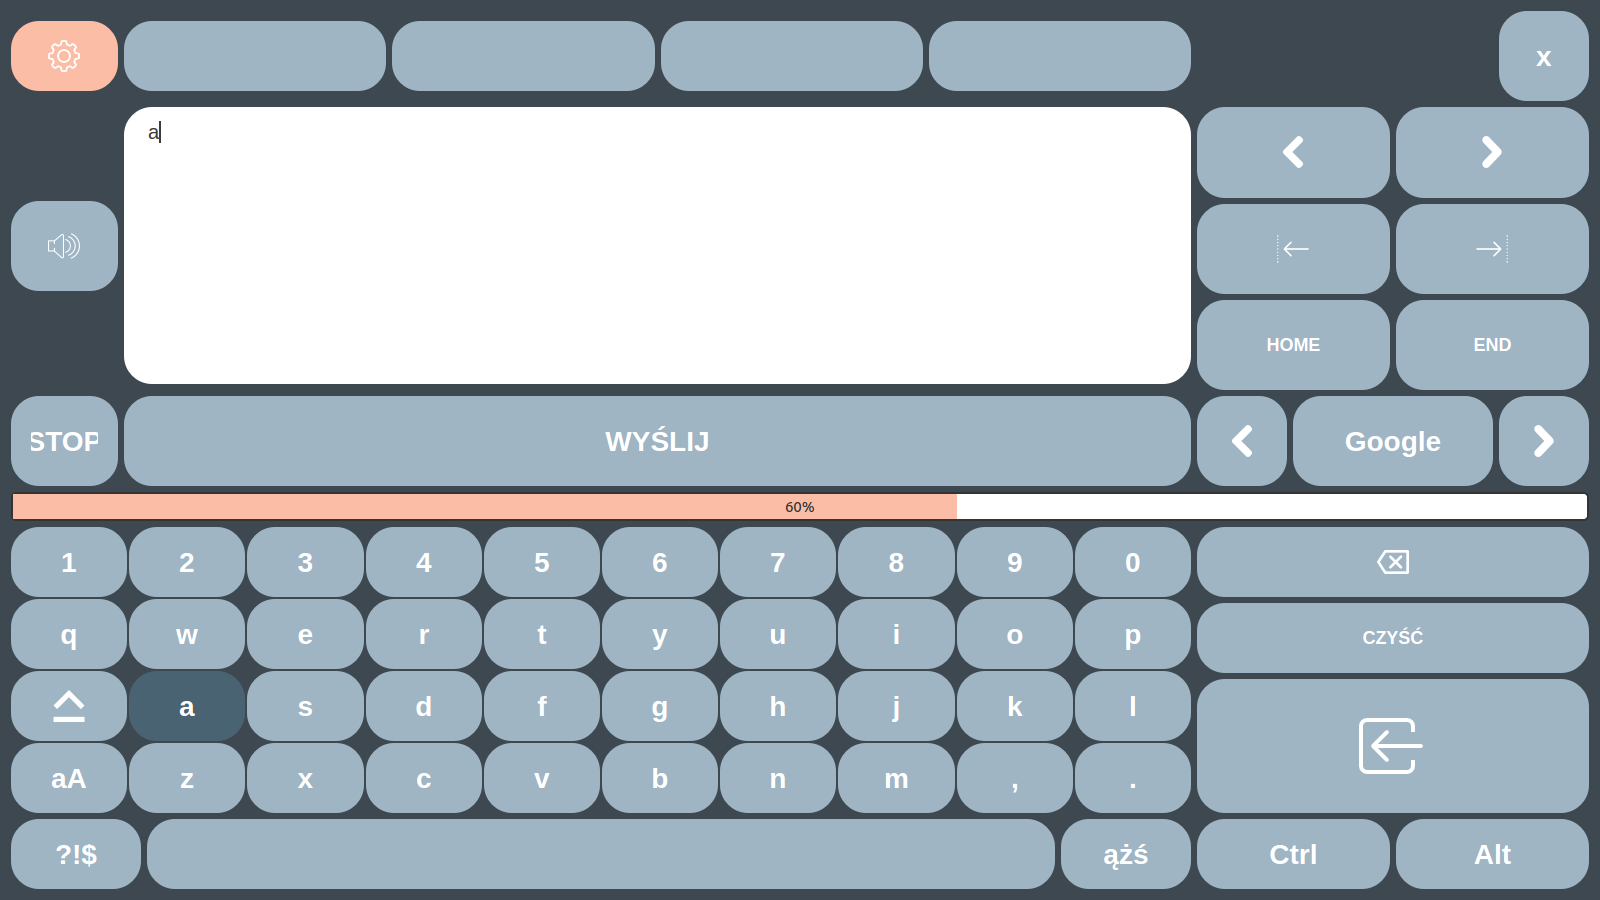
\includegraphics[width=1\textwidth]{img/startA.jpg}}
		\caption{Widok aplikacji z klawiatura w stanie zerowym po wpisaniu litery 'a'.}
		\label{fig:startA}
\end{figure}
\begin{figure}[!h]
		\centering
		\scalebox{.7}{
		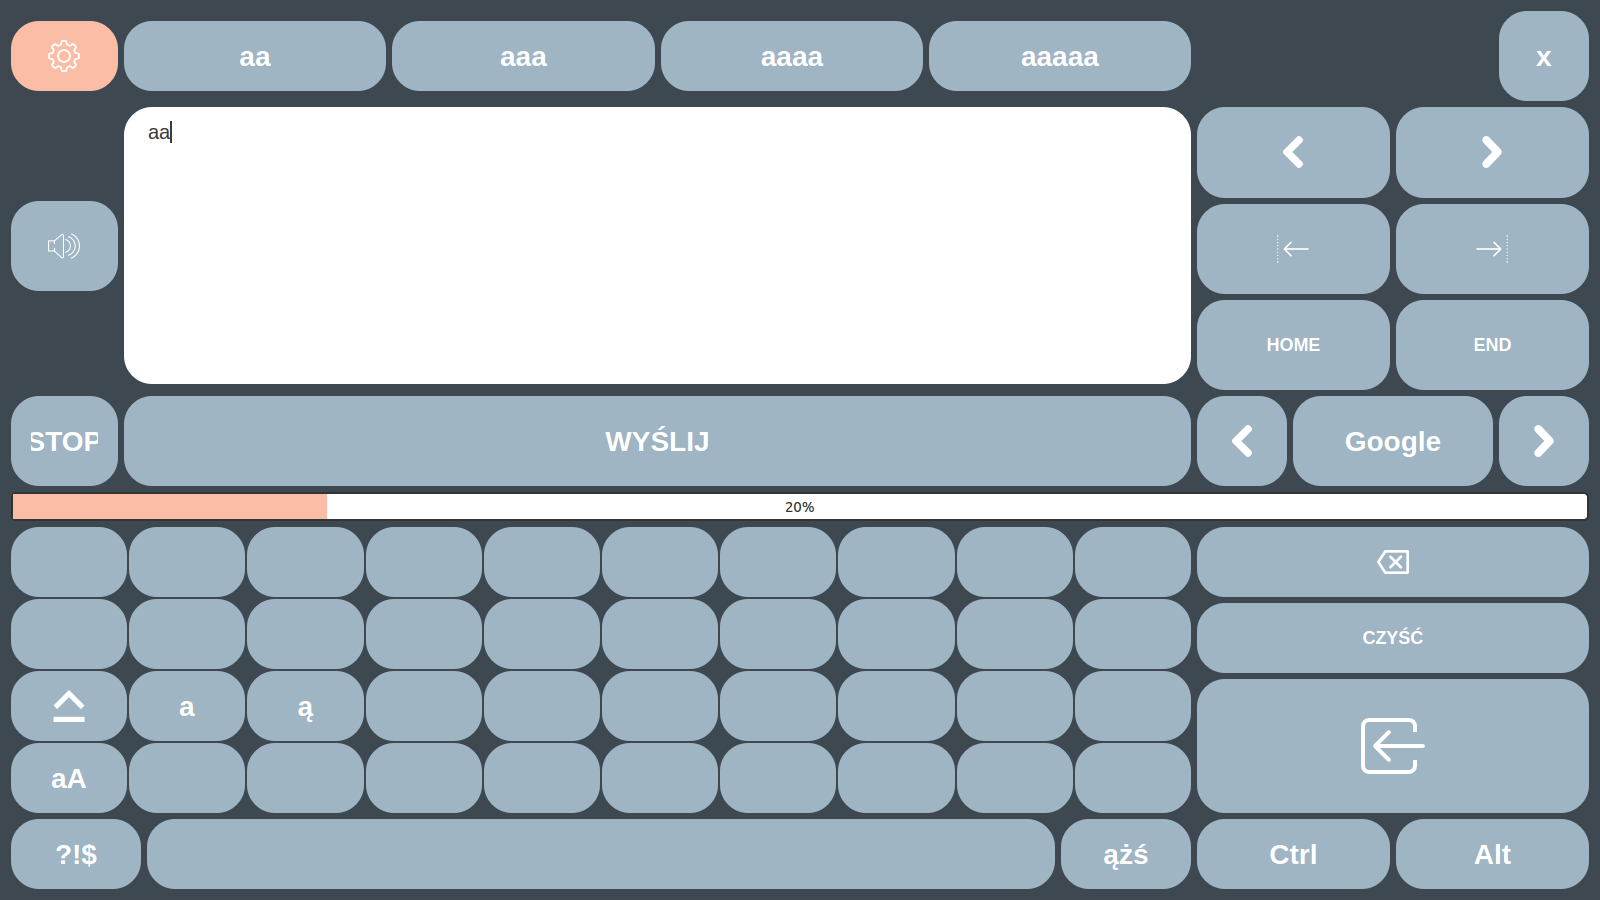
\includegraphics[width=1\textwidth]{img/doubleA.jpg}}
		\caption{Widok aplikacji z klawiaturą w stanie piątym po wpisaniu drugiej litery 'a'.}
		\label{fig:doubleA}
\end{figure}
W innym wypadku aktualna litera dopisywana jest do aktualnie tworzonoego słowa (currentWord), kursor przesuwany jest o jedną pozycję w prawo. Gdy dodana jest spacja aktualnie przetwarzane słowo jest uznawane za skończone i zapamiętywany jest nowy początek kolejnego słowa. Odświeżony zostaje również widok podpowiedzi, których powstawanie omówiono w późniejszym rozdziale ~\ref{sec:trietree}.
W sytuacji, gdy wybrana zostaje litera z menu kontekstowego (klawiatury w stanie piątym), to albo wpisany tekst zostaje podmieniony na polską literę,lub nie ulega zmianie. Przykładowo po wpisaniu ''aa'' użytkownik po raz kolejny wybiera literę ''a'' - tzn. planował wpisanie frazy ''aa''. Jeśli jednak decyduje się na literę ''ą'', to w miejsce widniejącego napisu ''aa'' pojawia się ''ą''.
Poglądowy diagram przepływu przedstawiono no rysunku ~\ref{fig:wordFlow}.
\begin{figure}[!h]
		\centering
		\scalebox{1}{
		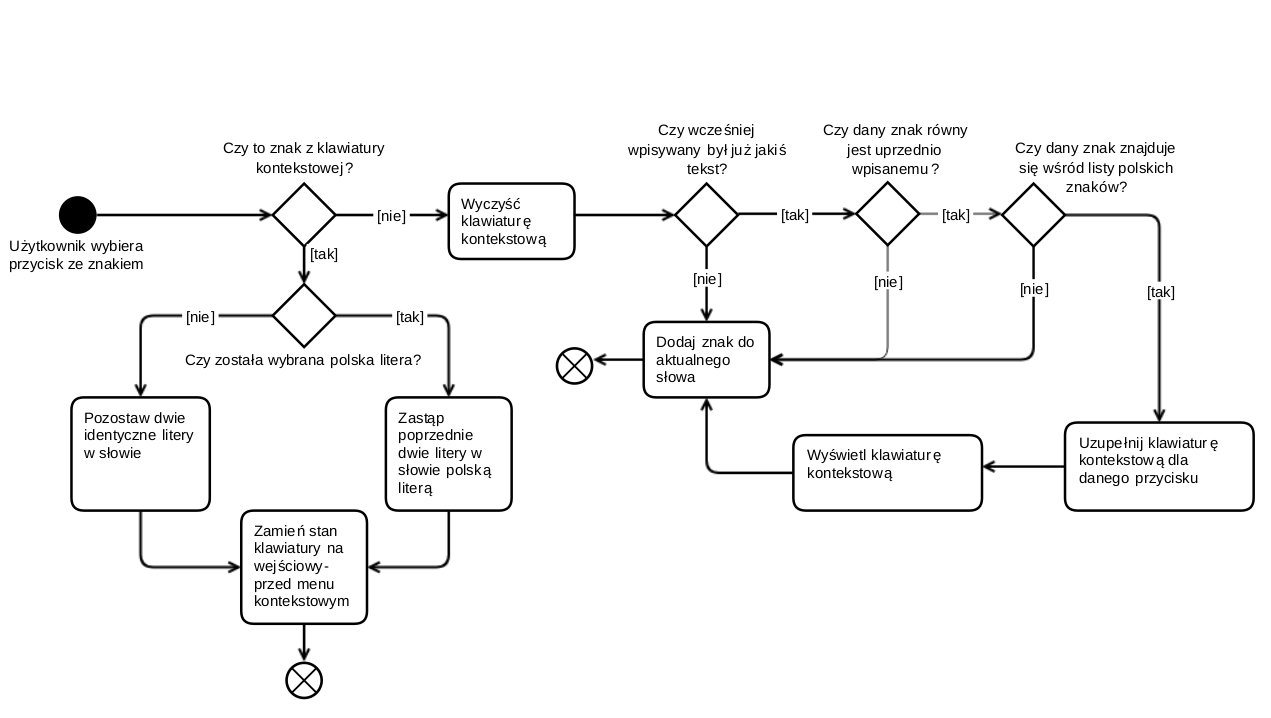
\includegraphics[width=1\textwidth]{img/writeFlow.jpg}}
		\caption{Widok aplikacji z klawiaturą w stanie piątym po wpisaniu drugiej litery 'a'.}
		\label{fig:wordFlow}
\end{figure}
\section{Praca z tekstem}~\label{sec:text}
Wpisywanie tekstu w aplikacji odbywa się poprzez specjalny algorytm kontrolujący zawartość aktualnie pisanego słowa oraz całego tekstu. Podczas każdej chwili działania programu w pamięci przechowywany jest currentWord, czyli aktualne słowo tj. ciąg znaków, liter lub cyfr, które zaczynają się na początku wpisywanego tekstu lub po spacji, a kończą się w pozycji kursora. Dodanie spacji po ciągu znaków kończy słowo i usuwa je ze zmiennej currentWord, a dodaje do zmiennej zwanej wholeText, która przechowuje dotychczas wpisany tekst. Przykładowo jeśli mamy tekst jak na rysunku ~\ref{fig:sentence} to w zmiennej wholeText przechowywujemy ''''Wymagajcie od bie choćby inni od was nie wymagali.'' ~Jan Paweł II '', a w currentWord ''sie''. W ten sposób podpowiedzi generowane będą jedynie dla cząstki ''sie'', a tekst wpisywany będzie w pozycji kursora, która również monitorowana jest przez zmienną currentPosition. Scalenie wholeText i currenWord następuję, gdy zmieniamy pozycję kursora strzałkami, lub jeśli do tekstu dodana zostanie spacja, a za kursorem nie znajduje się żaden znak przykładowo w takiej sytuacji znajdziemy się na rysunku ~\ref{fig:sentence2}. 
\begin{figure}[!h]
		\centering
		\scalebox{1}{
		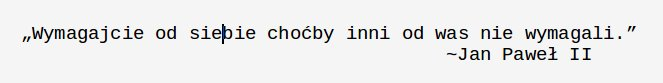
\includegraphics[width=1\textwidth]{img/sentence.jpg}}
		\caption{Przykład zapisywanie tekstu do zmiennych w zależności od pozycji kursora.}
		\label{fig:sentence}
\end{figure}
\begin{figure}[!h]
		\centering
		\scalebox{1}{
		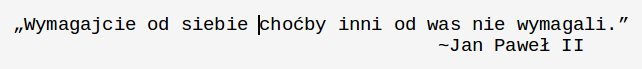
\includegraphics[width=1\textwidth]{img/sentence2.jpg}}
		\caption{Przykład zapisywanie tekstu do zmiennych w zależności od pozycji kursora.}
		\label{fig:sentence2}
\end{figure}

Zmienna currentWord została zespolona z wholeText poprzez wklenie jej na pozycji zapisanej jako currentWordStart. 
W celu dynamicznego ustalania pozycji currentWordStart oraz zawartości currentWord powstały funkcje: getCurrentWordStart() oraz getCurrentWord(). Działanie pierwszej zademonstrowano za pomocą pseudokodu ~\ref{sec:alg2}.
\begin{algorithm}
\caption{Działanie funkcji getCurrentWordStart()}
\label{sec:alg2}
\begin{algorithmic}
\IF{currentWord nie jest pusty \&\&  currentPosition nie jest  na początku tekstu}
\FOR{każda pozycja aż do początku tekstu}
\STATE pobierz literę z wholeText w danej pozycji
\IF{pobrana wartość nie jest liczbą ani literą}
\STATE $currentWordStart = dana pozycja + 1$
\ENDIF
\ENDFOR
\ENDIF
\end{algorithmic}
\end{algorithm}
Działanie drugiej sprowadza się do wycięcia faragmentu tekstu między currentWordStart, zaimplementowanym w wyniku działania poprzedniej funkcji, a currentPosition.


\section{Trie tree}\label{sec:trietree}
Jak wyżej ~\ref{sec:trie}  wspomniano, w pracy wykorzystano drzewo typu Trie w celu pracy z rozległym słownikiem. Słowa z pliku w formacie TXT wczytywane są do programu podczas uruchamiania klawiatury- każda z linii dostarczanego pliku powinna stanowić pojedynczy wyraz. Słowa te, za pomocą sztucznie wygenerowanych list kodujących oraz dekodujących polski alfabet, wprowadzane są do drzewa typu Trie. Drzewo takie powstaje poprzez stworzenie pustego węzła typu node - struktury zadeklarowanej w pliku nagłówkowym klasy obsługującej współpracę ze słownikiem – Dictionary. Struktura node przechowuje informacje o rodzicu bieżącego węzła, o jego potomkach – czyli węzłach następujących oraz wektor zawierający informację o przynależności danego węzła literowego do słowa. 
Po zainicjowaniu węzła zerowego, po kolei, analizowane są słowa ze słownika w funkcji insertWord().Każe jest rozpatrywane jako tablica liter (char) i iteracyjnie następuje najpierw kodowanie litery na odpowiadający jej indeks (za pomocą  mapy alfabet), potem, sprawdzane jest, czy drzewie nie istnieje już węzeł odpowiadający danej wartości. Gdy nie znaleziono gałęzi drzewa pasujących do poszukiwanej wartości tworzy się za pomocą funkcji calloc przestrzeń w pamięci na przyszłe dzieci tego węzła,a jako ich rodzica podaje się aktualnie przeglądany węzeł z literą. Kolejno, niezależnie od wyniku uprzednio rozpatrywanego warunku, o ile słowo wciąż posiada litery do przeglądu, przenosi się o poziom niżej w drzewie ( na poziom dziecka  uprzednio rozpatrywanej litery) i proces zachodzi od początku.  Gdy przetworzono wszystkie litery słowa do listy wystąpień ostatniego odwiedzonego węzła dopisany zostaje indeks słowa w słowniku – tym samym oznaczając jego koniec. W sposób graficzny przedstawiono działanie danej funkcji na rysunku ~\ref{fig:insertWord}
\begin{figure}[!h]
		\centering
		\scalebox{1}{
		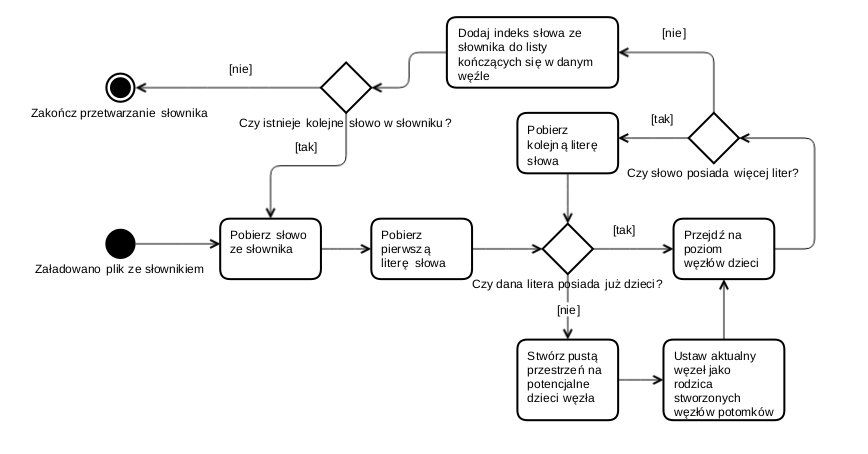
\includegraphics[width=1\textwidth]{img/insertWordFlow.jpg}}
		\caption{Diagram przepływu dla funkcji insertWord() wprowadzającej słowa do drzewa typu Trie. }
		\label{fig:insertWord}
\end{figure}

Po uzupełnieniu słownika można przejść do jego wykorzystywania - auto uzupełniania wpisywanego tekstu.
Każde wpisanie litery powoduje wywołanie metody updateHints(), która jest odpowiedzialna za tworzenie oraz wyświetlanie podpowiedzi, zgodnie z wprowadzonym do tej pory słowem. Jako poszukiwaną frazę traktujemy ciąg znaków, które użytkownik wpisał do pozycji kursora od ostatniej spacji, bądź początku tekstu. W wypadku, gdy ten ciąg znaków jest dłuższy niż dwa, wykorzystywana jest funkcja komunikująca się ze stworzonym słownikiem – searchWord(). Przekazywane jest drzewo Trie słownika oraz aktualnie poszukiwana fraza (bez formatowania). 
Wpisywana fraza, również traktowana jest jako zbiór liter, które przeglądane są jedna po drugiej. Dla każdej następuje zmiana dzięki mapie kodującej alfabet na odpowiadający indeks, który umożliwia przeszukiwanie słownika. Sprawdzane jest, czy istnieje potomek drzewa Trie o danym indeksie – jeśli tak, to następuje zmiana węzła na węzeł dziecka, tak, że przy przeszukiwaniu drzewa brane pod uwagę będą jedynie węzły z rodzicem będącym pierwszą literą poszukiwanej frazy. Gdy przeszuka się wszystkie litery, bądź w trakcie tego procesu zabraknie węzłów potomków dla danej kombinacji liter to zwracany jest odpowiednio ostatni węzeł wspólny dla danej frazy lub też węzeł pusty. Przykładowo - załóżmy, że mamy drzewo takie jak na rysunku ~\ref{fig:trie}. Jeśli wyszukamy frazę ''ko'' to funkcja wróci nam węzeł i jego dzieci - czyli możliwe auto uzupełnienia wyglądają tak jak na rysunku ~\ref{fig:trieKO}.
\begin{figure}[!h]
		\centering
		\scalebox{.5}{
		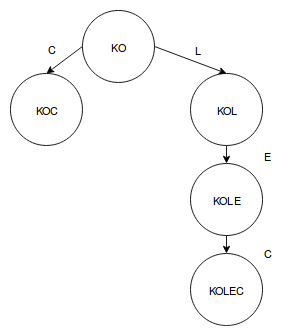
\includegraphics[width=1\textwidth]{img/trieKO.jpg}}
		\caption{Przykładowy węzeł do autouzupełniania słów po wpisaniu frazy ''ko''. }
		\label{fig:trieKO}
		\end{figure}
Złożenie końcówek wyrazów zachodzi w funkcji getSimilarEndings(), której przekazywany jest znaleziony
 węzeł, pusty wektor, do którego mają zostać zapisane wynikowe wyrazy oraz węzeł znaków niezbędny do dekodowania. 
W pierwszym kroku sprawdzane jest, czy w danym węźle kończą się  jakieś słowa, jeśli tak (wektor wystąpień węzła jest różny od zera), to każdą literę zapisaną w wyżej wymienionym wektorze znaków zapisuje się do jednego słowa (tworząc końcówkę do auto uzupełniania). Gotowy ciąg znaków zapisywany jest do wektora z końcówkami. W wypadku pierwszego wykonania się funkcji mamy do czynienia z pustym wektorem znaków- toteż nie zostanie stworzona żadna końcówka. Nawet jeśli  ‘’ko’’ było pełną formą słowa nie powinna ona się wyświetlać w proponowanych opcjach użytkownika. Aby uzupełnić wektor znaków należy przejrzeć przesłany węzeł (ten z rysunku ~\ref{fig:trieKO}) – w tym celu sprawdza się, czy dzieci węzła odpowiadającej każdej literze alfabetu nie są puste, gdyż programowe drzewo ma, prócz wcześniej przedstawionych gałęzi, jeszcze 33 (zakładając, że zaimplementowany alfabet posiada 35 liter) nieobdarzone wartością gałęzie przedstawione na rysunku ~\ref{fig:trieKOnull}. Gdy znaleziono element o niezerowej wartości pobierana jest za pomocą mapy symetrycznej (reverseAlfabet) wartość literowa węzła i wprowadzana jest do wektora znaków. Węzeł z ‘’ko’’ zmieniany jest węzeł pierwszego pierwszego dziecka – w tym wypadku ‘’koc’’. Następnie przez rekurencję ponownie rozpoczyna się sprawdzanie, czy dane słowo kończy się w tym węźle, jeśli tak to proces zachodzi według powyżej opisanych kroków, jeśli nie to znów poszukiwany jest węzeł potomny z kolejną literą końcówki słowa do auto uzupełniania. Algorytm przedstawiono w sposób graficzny na rysunku ~\ref{fig:similarEndingsFlow}
		\begin{figure}[!h]
		\centering
		\scalebox{.9}{
		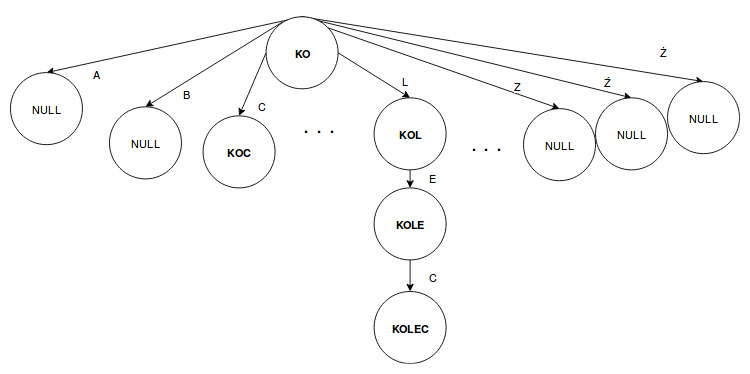
\includegraphics[width=1\textwidth]{img/trieKOnull.jpg}}
		\caption{Reprezentacja przykładowego węzła widzianego w programie. }
		\label{fig:trieKOnull}
		\end{figure}
				\begin{figure}[!h]
		\centering
		\scalebox{1}{
		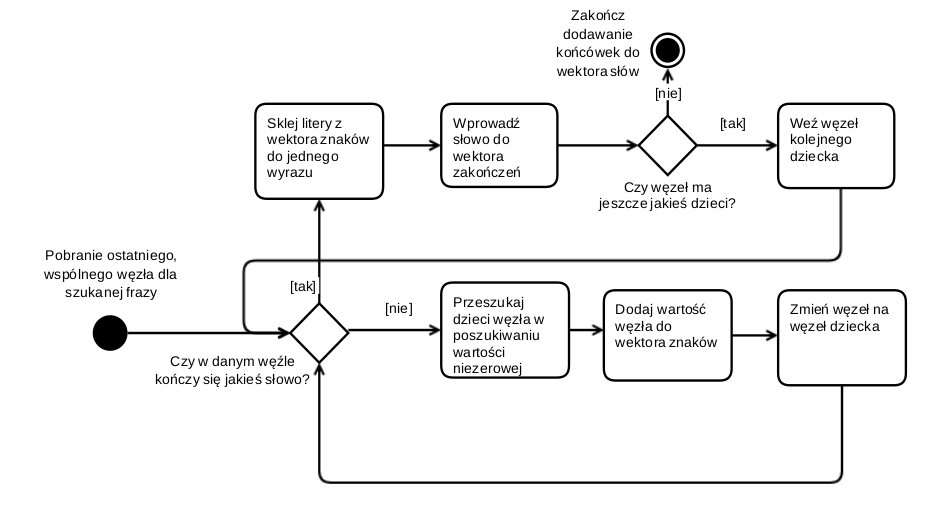
\includegraphics[width=1\textwidth]{img/similarEndingsFlow.jpg}}
		\caption{Diagram przepływu dla funkcji getSmiliarEndings().}
		\label{fig:similarEndingsFlow}
		\end{figure}
Ostatnim krokiem w stworzeniu podpowiedzi jest skrócenie listy końcówek do liczby przycisków przeznaczonych na podpowiedzi oraz zespolenie ich z dotychczas wpisanym słowem. Taki ciąg znaków można przedstawić użytkowniku jako napis na przycisku, który po wybraniu wpisuje reprezentowany tekst do pola tekstowego zamieniając dotychczasową frazę na wybraną oraz dodając znak spacji na końcu nowowybranego słowa.

\section{Google Api}


\end{document}